With differentials of smooth functions at hand, we are ready to discuss submanifolds: smaller manifolds sitting inside larger ones.
We have already seen an example at the begininng of the course.
In Exercise~\ref{exe:subsetsmanifolds}, we proved that any open subset $U\subseteq M$ can be made into a smooth manifold with a differentiable structure induced by the one of $M$.
These, somehow trivial, submanifolds are called \emph{open submanifolds}.
Bu there are many other examples beyond these ones.
In fact, you may have already seen them in multivariable analysis.

In this chapter we will briefly explore what subsets of manifolds are still manifolds of their own rights, how their topologies are related and how their smooth structures are related.
We will conclude the chapter answering the question opened at the beginning of the previous chapter: do tangent spaces really coincide with the intuitive understanding of a tangent hyperplane to a point on the manifold?

\begin{marginfigure}
  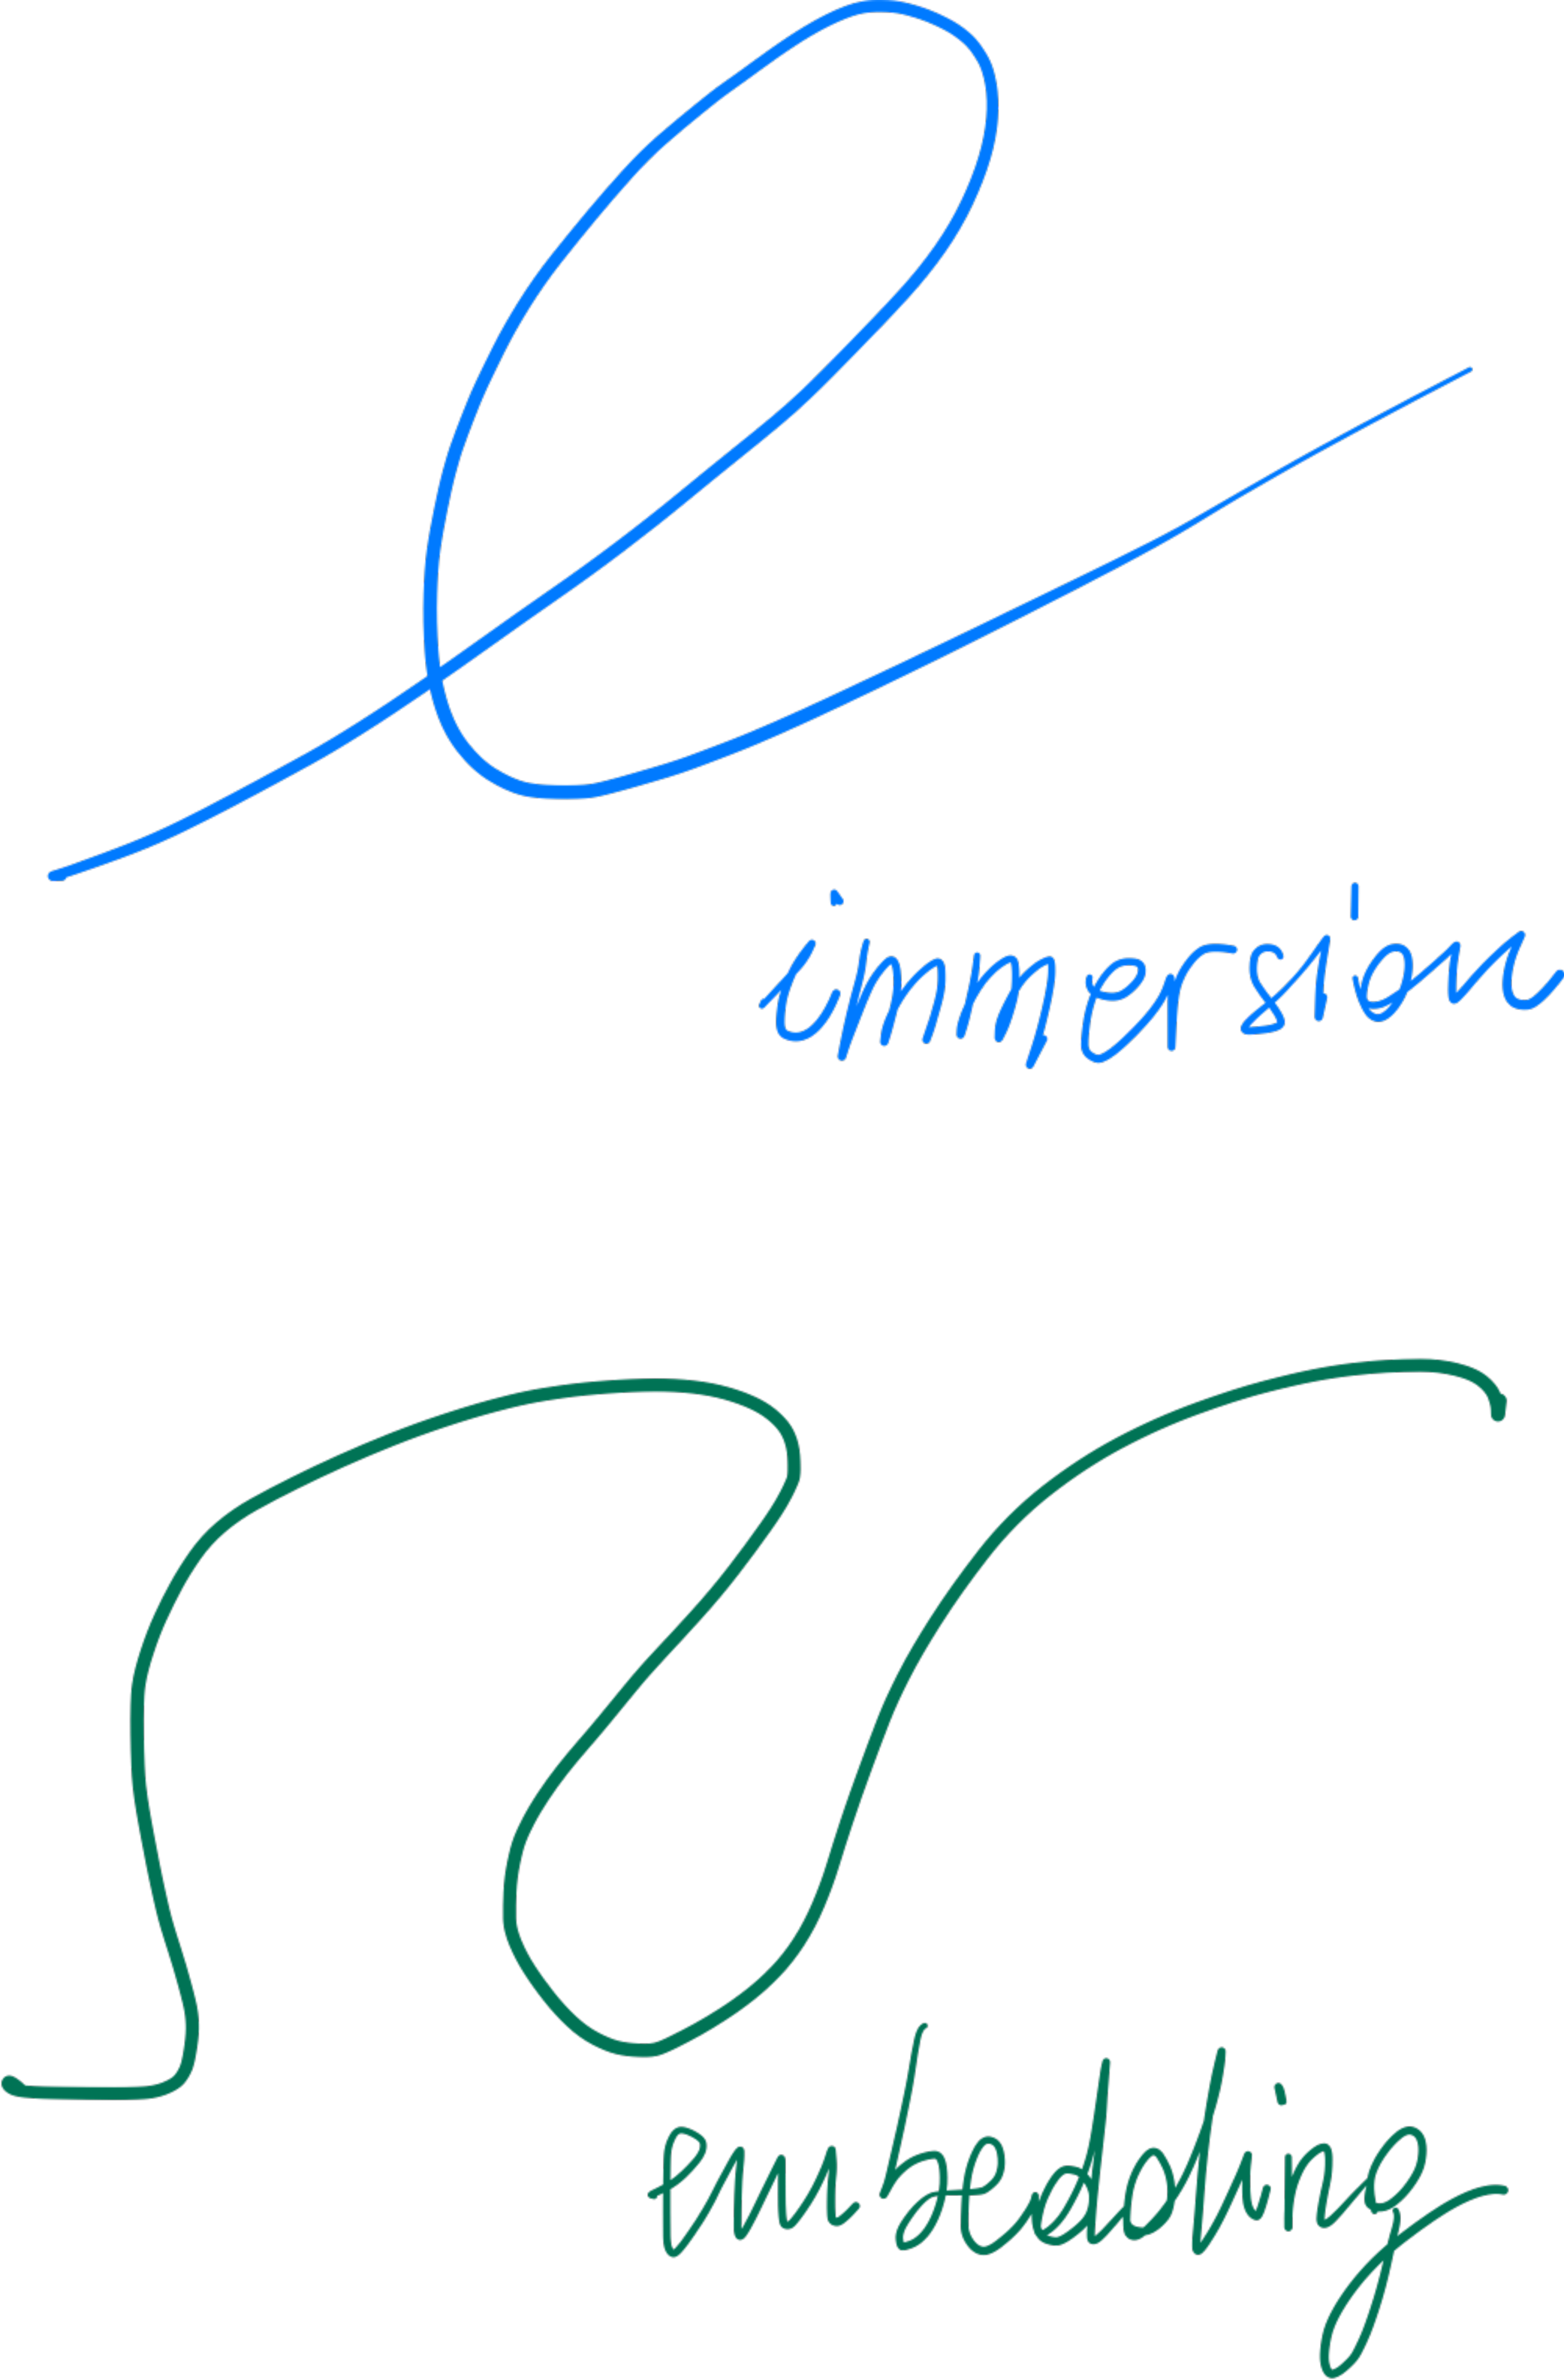
\includegraphics{2_8_1-immersion-embedding}
\end{marginfigure}
\begin{definition}
  Let $M^m$ and $N^n$ be differentiable manifolds and $F:M\to N$ a smooth function.
  \begin{itemize}
    \item $F$ is a \emph{immersion} if $dF_p$ is injective for all $p\in M$ ($\Rightarrow\; m\leq n$);
    \item $F$ is a \emph{submersion} if $dF_p$ is surjective for all $p\in M$ ($\Rightarrow\; m\geq n$);
    \item $F$ is a \emph{embedding}\footnote{This is a particular case of a more general concept, the topological embedding, which defined as an injective continuous map that is a homeomorphism onto its image.} if $F$ is an injective immersion that is also a homeomorphism onto its range $F(M)\subset N$, where the topology on $F(M)$ is the subspace topology as a subset of $N$.
  \end{itemize}
\end{definition}

\begin{example}
  \begin{enumerate}
    \item The prototype of an immersion is the inclusion of $\R^m$ in a higher-dimensional $\R^n$:
          \begin{align}
            i & : \R^m \hookrightarrow \R^n,                                                                                 \\
            i & : \left(x^1, \ldots, x^m\right) \mapsto \left(x^1, \ldots, x^m, \LaTeXunderbrace{0, \ldots, 0}_{n-m}\right).
          \end{align}

          Indeed, the $n\times m$ matrix
          \begin{equation}
            di_x = Di(x)
            = \begin{pmatrix}
              1      & 0      & \cdots & 0      \\
              0      & 1      & \cdots & 0      \\
              \vdots &        & \ddots & \vdots \\
              0      & \cdots & \cdots & 1      \\
              0      & \cdots & \cdots & 0      \\
              \vdots &        &        & \vdots \\
              0      & \cdots & \cdots & 0
            \end{pmatrix}
          \end{equation}
          has full rank (equal to $m$) and is therefore injective.
          Moreover, the map $i$ is injective and continuously invertible on its range, so it is also an embedding.

    \item The prototype for a submersion is the projection of $\R^m$ onto a lower-dimensional $\R^n$: $\pi\left(x^1,\ldots,x^n,x^{n+1},\ldots,x^m\right) = \left(x^1,\ldots,x^n\right)$.

          Indeed, the $n\times m$ matrix
          \begin{equation}
            d\pi_x = D\pi(x)
            = \begin{pmatrix}
              1      & 0      & \cdots & 0      & 0      & \cdots & 0      \\
              0      & 1      & \cdots & 0      & \vdots &        & \vdots \\
              \vdots &        & \ddots & \vdots & \vdots &        & \vdots \\
              0      & \cdots & \cdots & 1      & 0      & \cdots & 0
            \end{pmatrix}
          \end{equation}
          has full rank (equal to $n$) and is therefore surjective.
          Hence, $i$ is a submersion.

    \item Let $m=1$, $n > 1$ and $\gamma:\R\to\R^n$ a smooth curve.
          The map $\gamma$ is an immersion if and only if its velocity vector satisfies $\gamma'(t)\neq0$ for all $t\in\R$.
          If the curve intersects itself, e.g $f(t_1) = f(t_2)$ for some $t_1\neq t_2$, then $f$ is not an embedding.
  \end{enumerate}
\end{example}

\begin{remark}
  Surjectivity of submersions or injectivity of immersions are properties of the differentials, not of the maps themselves.
  %
  For example, if $U\subset M$ open, the inclusion $i: U \to M$ is both an immersion and a submersion.
\end{remark}

\begin{definition}
  Let $M$ and $N$ smooth manifolds such that $M\subset N$ as a set.
  We say that $M$ is an \emph{embedded (or regular) submanifold} of $N$ if the inclusion $M\hookrightarrow N$ is an embedding. If the inclusion is just an immersion, we say that $M$ is an \emph{immersed submanifold}.
\end{definition}

This definition already hints to the fact that smooth maps are going to be usefulin providing ways to nicely include a manifold into the another and in giving new ways to construct manifolds in the first place.
In the rest of this chapter we will try to give an answer to the following questions:
\begin{itemize}
  \item if $F$ is an immersion, what can we say about its image $F(M)$ as a subset of $N$?
  \item if $F$ is a submersion, what can we say about its levelsets $f^{-1}(q) \subset M$?
\end{itemize}
And what can we say about the corresponding tangent spaces?

Before moving on, it is useful to recall some results from multivariable analysis.
A function $f:\R^m \to \R^n$ between euclidean spaces has rank $k$ at $x\in\R^m$ if its ($n\times m$) Jacobian matrix $Df(x)$ has rank $k$.
The function has \emph{maximal rank}\footnote{Alternatively, it is of \emph{full rank}.} at $x$ if $k = \min(n,m)$.
When $n=m$, $f$ has maximal rank at $x$ if and only if the square matrix $Df(x)$ is an invertible matrix.

As for many local properties, this definition carries over to manifolds rather ``smoothly''.

\begin{definition}
  A smooth map $F:M\to N$ has \emph{rank $k$} at a point $p$ if its differential $dF_p$ has rank $k$, that is, if the linear subspace $dF_p(T_pM)$ has dimension $k$ inside $T_{F(p)}N$.
\end{definition}

And the same is true for the inverse function theorem:
compare the following statements.

\begin{theorem}[Inverse function theorem]\label{thm:ift}
  Let $U\subset\R^n$ open and $f:U \to \R^n$ be a smooth map.
  Assume that $f$ has maximal rank at some $x\in U$, then there exists an open neighbourhood $\Omega\subset U$ of $x$ such that  $f\big|_\Omega : \Omega \to f(\Omega)$ is a diffeomorphism.
\end{theorem}

\begin{theorem}[Inverse function theorem for manifolds]\label{thm:iftm}
  Let $F:M\to N$ be a smooth function between smooth manifolds of the same dimension $n$.
  Let $p\in M$ and assume that $F$ has maximal rank (i.e. rank $n$) at $p$.
  Then there exists an open neighbourhood $V$ of $p$ such that the restriction $F:V\to F(V)$ is a diffeomorphism.
\end{theorem}
% \begin{proof}
%   This is a purely local statement.
%   Let $(U,\varphi)$ be a chart about $p\in M$ and let $(V, \psi)$ be a chart about $F(p)\in N$.
%   Since both $\varphi$ and $\psi$ are diffeomorphisms (and thus have maximal rank), the derivative of
%   \begin{equation}
%     \psi \circ F \circ \varphi^{-1}: \varphi(U\cap F^{-1}(V)) \to \psi(F(U)\cap V)
%   \end{equation}
%   has rank $n$ at $\varphi(p)$.
%   Thus the inverse function theorem, Theorem~\ref{thm:ift}, there exists $\Omega \subset \varphi(U\cap F^{-1}(V))$ such that $\psi \circ F \circ \varphi^{-1}\big|_{\Omega}$ is a diffeomorphism.
%   Therefore, once again since both $\varphi$ and $\psi$ are diffeomorphisms, $F\big|_W : W \to F(W)$ is also a diffeomorphism for $W := \varphi^{-1}(\Omega)$.
% \end{proof}
\begin{exercise}
  Use the euclidean inverse function theorem (Theorem~\ref{thm:ift}) on $\R^n$ to prove Theorem~\ref{thm:iftm}.
\end{exercise}


In fact, also analogues of the implicit function theorem carry over.
We will state them without going into the details of the proofs.

\begin{marginfigure}
  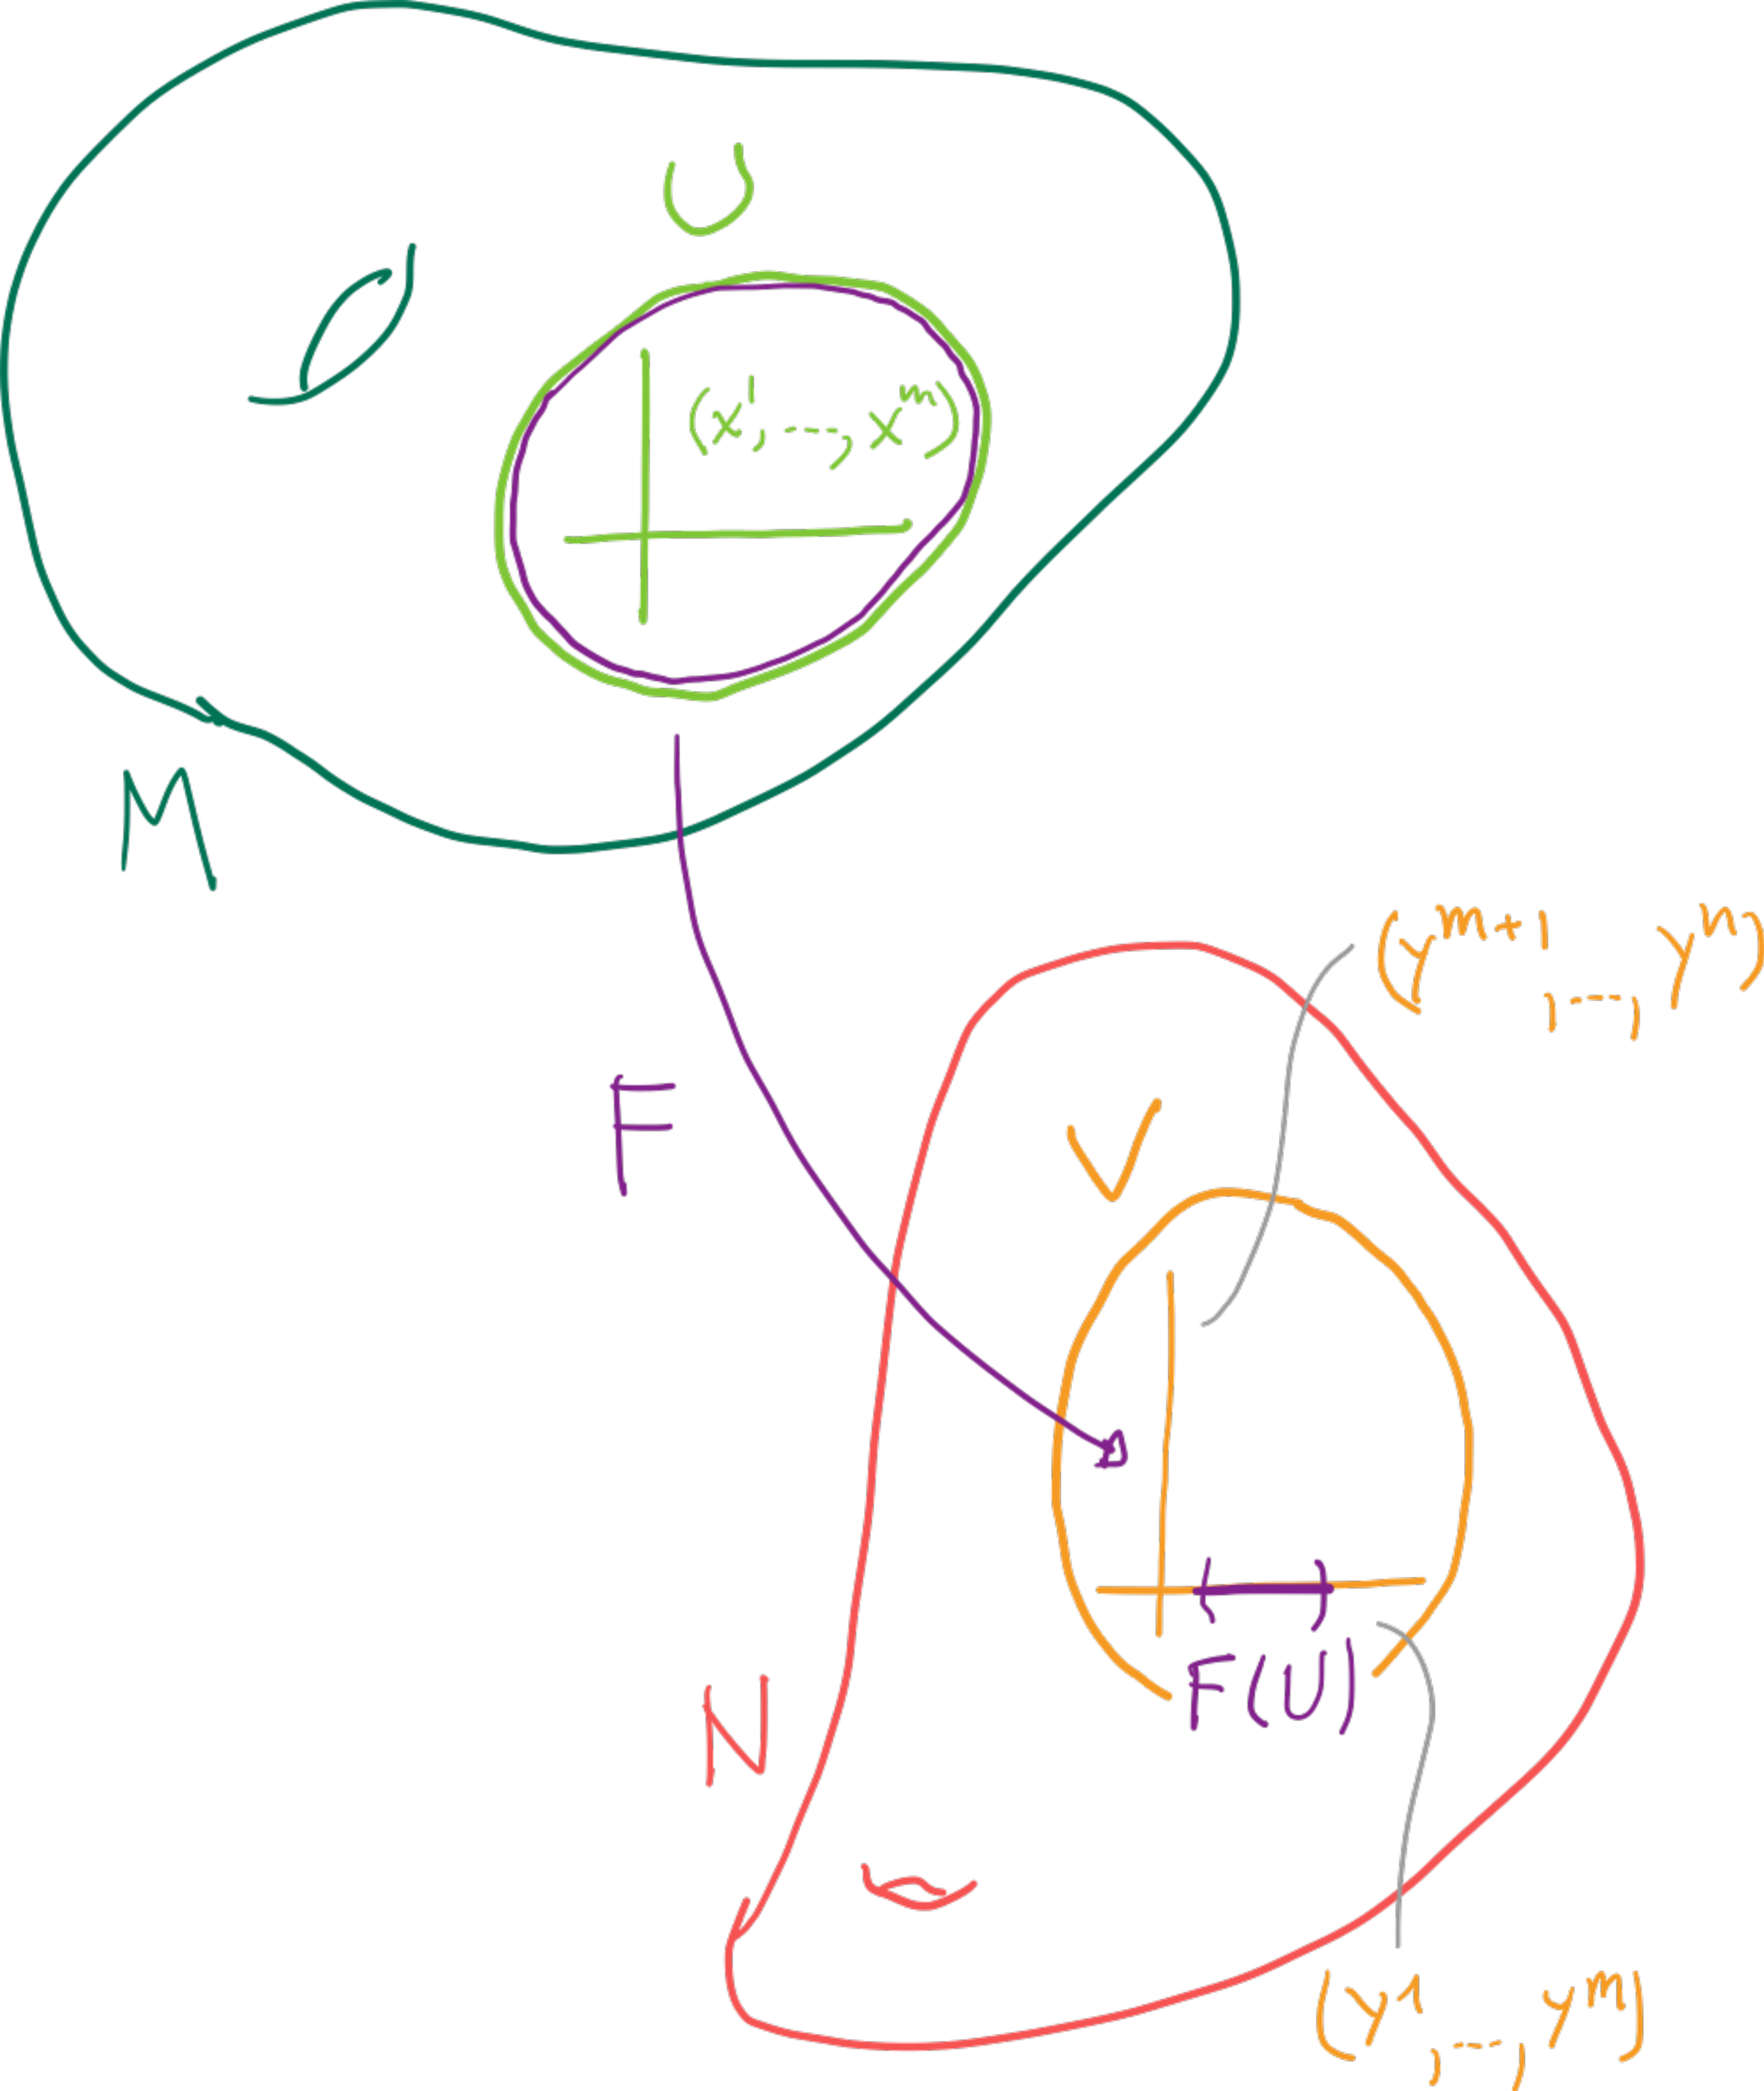
\includegraphics{2_8_9-mapping.pdf}
  \caption{Theorem~\ref{prop:slice_chart} in a picture.}
\end{marginfigure}
\begin{proposition}\label{prop:slice_chart}
  Let $M^m$ and $N^n$ be smooth manifolds and $F:M\to N$ an immersion.
  Then for any $p\in M$, there exists a neighbourhood $U$ of $p$ and a chart $(V,\psi)$ about $F(p)\in N$ such that
  \begin{enumerate}[(i)]
    \item If $y^i = r^i\circ \psi$ are the local coordinates of $\psi$ then
          \begin{equation}\label{eq:slice_chart}
            F(U)\cap V = \left\{ q \in V \;\mid\; y^{m+1}(q)=\cdots=y^n(q)=0\right\};
          \end{equation}
    \item $F\big|_U$ is an embedding.
  \end{enumerate}
\end{proposition}

If $F$ is an embedding, and this $M$ is an embedded submanifold, then the set $F(U)$ above can be written as $F(U) = F(M)\cap W$ for some open set $W\subset N$.
By replacing $V$ in~\eqref{eq:slice_chart} with $V\cap W$, one gets
\begin{equation}
  F(M)\cap V = \left\{ q \in V \;\mid\; y^{m+1}(q)=\cdots=y^n(q)=0\right\}.
\end{equation}
In particular, this means that a $m$-dimensional submanifold is also a $m$-dimensional manifold whose charts are the ones above after we drop the final $n-m$ components.

The proposition above shows that an immersion is always a local embedding.
\begin{exercise}
  \begin{enumerate}
    \item If $M$ is compact, an injective immersion $F:M\to N$ is always an embedding.
    \item This is not necessarily the case in the non-compact case, give a counterexample.
  \end{enumerate}
\end{exercise}

\begin{lemma}
  With the notation of Proposition~\ref{prop:slice_chart}, assume that around any point $p\in M$ there is a chart of the form
  \begin{equation}
    M\cap V = \left\{ q \in V \;\mid\; y^{m+1}(q)=\cdots=y^n(q)=0\right\} \subset N.
  \end{equation}
  Then, if we endow $M$ with the subspace topology on $N$, $M$ is a topological manifold of dimension $m$.
  Furthermore, it has a smooth structure that makes it into an embedded submanifold of $N$.
\end{lemma}
\begin{proof}[Sketch]
  Let $\pi: \R^n\to\R^m$ be the projection as in the examples above.
  Let $p\in M$ and let $(V,\psi)$ be a chart with coordinates $(y^i)$ of the form above.
  If we endow $M$ with the subspace topology, then $\sigma:= \pi \circ \psi\big|_{M\cap V}$ is a homeomorphism.
  Repeating this at any point we end up with a collection of maps satisfying the hypotheses of Lemma~\ref{lem:manifold_chart}.
  Thus $M$ is a smooth manifold of dimension $n$ and its topology coincides with the subspace topology.

  Finally, with the inclusion $i:M\hookrightarrow N$ one has that $\psi \circ i\circ \sigma^{-1} (p^1,\ldots,p^n) = (p^1,\ldots,p^n,0,\ldots,0)$ which is smooth.
\end{proof}

A non-trivial consequence of the previous lemma is the following proposition\footnote{Refer to \cite[Proposition 5.8 and Proposition 5.31]{book:lee}.}.

\marginnote[1em]{In Proposition~\ref{prop:uniqdiffeoinclusion} it is not enough to ask that $\iota$ is smooth! As counterexample consider the two manifolds $(\R, \cA_1)$ with $\cA_1 := \{(\R, \id_\R)\}$ and $(\R, \cA_2)$ with $\cA_2 := \{(\R, x\mapsto x^3)\}$. The inclusion of open sets in $\R$ is smooth in both cases but is a diffeomorphism only in one.}
\begin{proposition}\label{prop:uniqdiffeoinclusion}
  Let $M$ be a smooth manifold and $U\subset M$ an open set.
  Then $U$ has a unique differentiable structure such that the inclusion $\iota:U\hookrightarrow M$ is a diffeomorphism.
\end{proposition}

\newthought{Up to this point}, the first manifold either had the same dimension or was smaller than the second one.
What if it is larger?

\begin{definition}
  Let $F:M^m \to N^n$, $m\geq n$, be a smooth map between smooth manifolds.
  A point $p\in M$ is said to be a \emph{regular point} of $F$ if $dF$ has rank $n$ at $p$, while it is called a \emph{critical point} if it is not.

  Similarly, a point $q\in N$ is called a \emph{regular value} if every point in $F^{-1}(q)$ is a regular point, and \emph{critical value} otherwise. If $q\not\in F(M)$, then $q$ is considered a regular value (in the sense that there is nothing to check in its preimage by $F$).
  Cf. Figure~\ref{fig:2_8-crit_pts}.
\end{definition}
\begin{marginfigure}
  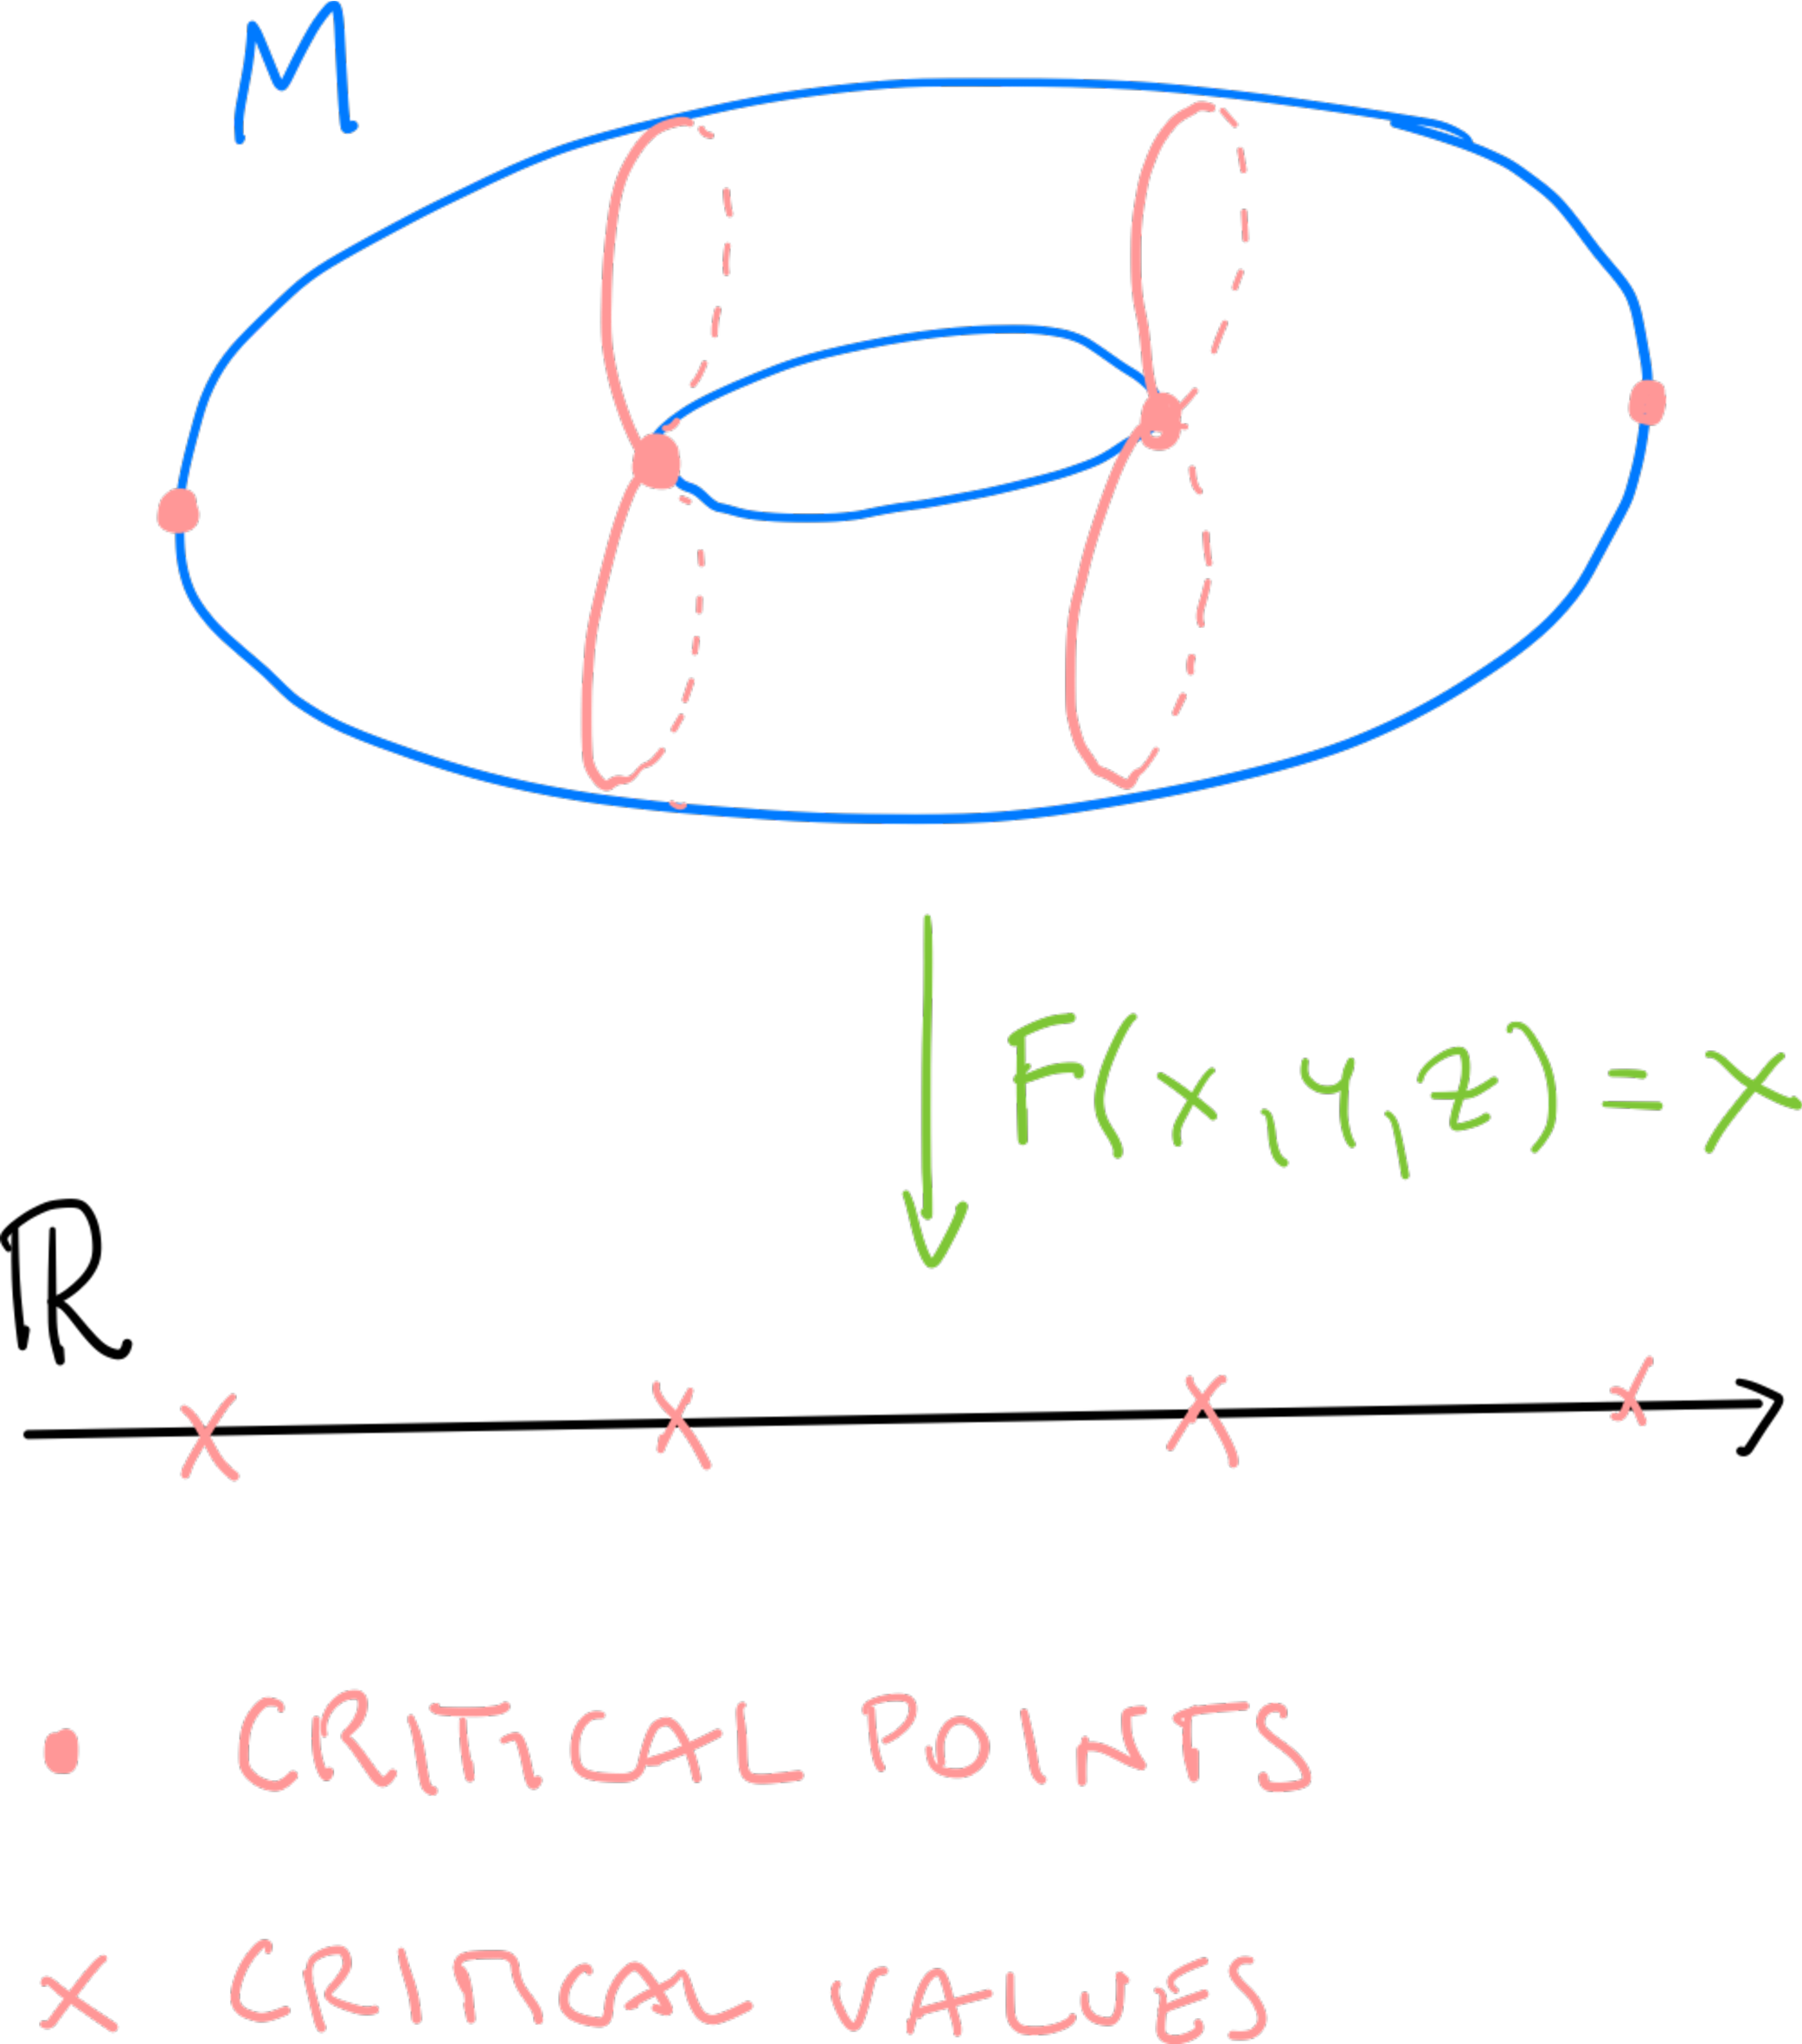
\includegraphics{2_8-crit_pts.pdf}
  \caption{Beware of the subtleties here. The map $F=\pi_x\circ i$ for the inclusion $i:\bT^2\hookrightarrow\R^3$ and the projection $\pi_x(x,y,z)=x$.
    So $dF_p = d (\pi_x)_{i(p)} \circ d i_p$. The latter is zero if the image of $T_p\bT^2$ by $d i_p: T_p\bT^2\hookrightarrow T_p\R^3$ is contained in the $yz$-plane (the reason will be clear by the end of the chapter): the critical points depicted here are exactly those points for which the tangent plane is the $yz$-plane.}
  \label{fig:2_8-crit_pts}
\end{marginfigure}

With this definition at hand, we are ready to state one of the most important theorems in this lecture.
Differently from most previous ones, the statement is not local.

\begin{theorem}[Implicit function theorem for manifolds]\label{thm:impl_fun}
  Let $m\geq n$ and let $F: M^m \to N^n$ be a smooth map between smooth manifolds.
  If $q\in N$ is a regular value of $F$ and $P := F^{-1}(q)$ is not empty, then $P$ is a topological manifold of dimension $m-n$.
  Moreover, there exists a smooth structure on $P$ which makes it into a smooth embedded submanifold of $M$.
\end{theorem}

\begin{remark}
  If $F:M\to N$ is a submersion, Theorem~\ref{thm:impl_fun} implies that any $p\in M$ belongs to the $(m-n)$-dimensional embedded submanifold $F^{-1}(F(p))$.
\end{remark}

We can gather this observation and the previous results (the inverse and the implicit function theorems) into the following proposition (of which we are also omitting the proof).

\begin{proposition}\label{prop:submanifolds_and_R}
  The following assertions are equivalent.
  \begin{enumerate}[(i)]
    \item $P^n\subset M^m$ is a $n$-dimensional submanifold\footnote{So, $n \leq m$.}.
    \item $P$ is locally the image of an embedding of a subset of $\R^n$.
          That is, for every $p\in P$ there exists $g\subset P$ open neighbourhood of $p$, an open set $U\subset\R^n$ and an embedding
          \begin{equation}
            \varphi : U \to M \quad\mbox{such that}\quad \varphi(U)=V.
          \end{equation}
    \item $P$ is locally a level set of a submersion into $\R^{m-n}$.
          That is, for every $p\in P$ there exists $V\subset P$ open neighbourhood of $p$ and a submersion $\psi: V \to\R^{m-n}$ such that
          \begin{equation}
            M\cap V = \{q\in V \;\mid\; \psi(q) = 0\}.
          \end{equation}
  \end{enumerate}
\end{proposition}

\begin{remark}\label{rmk:WhitneyET}
  Whitney Embedding Theorem states that any smooth $n$-dimensional manifold can be smoothly embedded into $\R^{2n}$.
  Thus any abstract manifold is diffeomorphic to a submanifold of $\R^m$ (for some $m$).
\end{remark}

\begin{remark}
  The concepts expressed in this section are extremely relevant in the contexts of mechanics and topology.
  Some good keywords to know more, here, could be Morse Theory, Floer Homology or Arnold's conjecture.
  We will not get into this, but I will refer you to a nice article from Quanta magazine that touches upon these topics \cite{article:quanta:floer}.
\end{remark}

\begin{example}\label{ex:s2}
  The sphere $\bS^2 = \{x\in\R^3 \mid \|x\| = 1\}$ is a $2$-dimensional submanifold of $N=\R^3$.
  This is immediate using the third condition in the Proposition~\ref{prop:submanifolds_and_R}: let $\psi(x) = \|x\|^2 -1 : \R^3 \to \R$, then $\psi$ is smooth, $\bS^2 = \{x\in\R^3\mid\psi(x)=0\}$ and, denoting $t$ the coorindates on $\R$, $d\psi_x(v)= v^i \frac{\partial \psi}{\partial x^i}|_x \frac{\partial}{\partial t}|_0 = (2x\cdot v) \frac{\partial}{\partial t}|_0$, that is, as a 1x3 matrix $d\psi_x = 2(x^1\; x^2\; x^3)$ so it is of maximal rank $1$ for all $x\in\bS^2$.
\end{example}

\begin{example}
  Let $N = \R^2$ and $P = \{ x\in N \;\mid\; x^2 = |x^1| \}$.
  Then $P$ is \emph{not} a submanifold, but it can be equipped with a manifold structure.
  For example with the global atlas $\{(P,\; (x^1,x^2)\mapsto x^1)\}$, $P$ is a manifold diffeomorphic to $\R$.
\end{example}

\begin{exercise}
  A real-valued function $f:M\to\R$ on a manifold has a local maximum at $p\in M$ if there is a neighbourhood $U\subset M$ of $p$ such that $f(p) \geq f(q)$ for all $q\in U$.
  \begin{enumerate}
    \item Show that if a differentiable function $f:(a,b)\to\R$, has a local maximum at $x\in (a,b)$, then $f'(x) = 0$.
    \item Prove that a local maximum of a function $f\in C^\infty(M)$ is a critical point of $f$.\\
          \textit{\small Hint: choose $X_p\in T_pM$ and let $\gamma(t)$ be a curve in $M$ starting at $p$ with initial velocity $X_p$. The $f\circ \gamma$ is a real-valued function with local maximum at $0$...}
  \end{enumerate}
\end{exercise}

\newthought{We still have a question pending} since the beginning of the previous chapter.
Is the tangent space to a sphere the one that we naively imagine (see Figure~\ref{fig:tan-embedded-sphere})?
To finally answer the question, we will prove one last proposition.

\begin{proposition}
  Let $F:M^m\to N^n$ be a smooth map between smooth manifolds.
  Let $q\in N$ be a regular value of $F$ such that $P:=F^{-1}(q)\neq\emptyset$ and let $i:P\hookrightarrow M$ denote the inclusion.
  Then, for all $p\in P$, one has
  \begin{equation}
    d i_p(T_p P) = \ker dF_p.
  \end{equation}
\end{proposition}
\begin{proof}
  Both $d i_p(T_p P)\subset T_p M$ and $\ker dF_p \subset T_p M$ are linear subspaces of the same dimension $m-n$, therefore we only need to show that one contains the other, e.g. $d i_p(T_p P) \subset \ker dF_p$.

  Take $f\in C^\infty(N)$ and $v\in T_p P$. By the chain rule\footnote{Proposition~\ref{thm:chainrule_mfld}} we get
  \begin{align}
    (d F_p \circ d i_p)(v)(f) = d(F\circ i)_p(v)(f) = v(f\circ F\circ i).
  \end{align}
  Since $F\circ i\big|_{P} \equiv q$ constant, $f\circ F\circ i\in C^\infty(P)$ is the constant function $p \mapsto f(q)$ and by Corollary~\ref{cor:derzero} we have $v(f\circ F\circ i)=0$.
\end{proof}

\begin{example}
  We have seen in Example~\ref{ex:s2} that $\bS^2 = F^{-1}(0)$ is a smooth manifold of dimension $2$.
  Denoting the inclusion by $i:\bS^2 \hookrightarrow\R^3$, one has
  \begin{equation}\label{ex:tan_sph}
    di_p(T_p\bS^2) = \cT_p(p^\perp)
  \end{equation}
  where $\cT_p:\R^3\to T_p\R^3$ is the map defined in Exercise~\ref{ex:tg_curve_iso} and
  \begin{equation}
    p^\perp := \big\{q\in\R^3 \;\mid\; \left\langle p, q\right\rangle = 0\big\},
  \end{equation}
  where $\left\langle\cdot,\cdot\right\rangle$ is the usual euclidean dot product. The latter directly comes from computing $dF_p$ and its kernel, which we essentially already did in Example~\ref{ex:s2}.
  Take a long deep breath and unfold the definitions in~\eqref{ex:tan_sph}, here it may be useful to draw a picture\footnote{Which is generally always the case in geometry and topology, and most other mathematical fields.}.
  Equation~\eqref{ex:tan_sph} implies that the tangent space to $\bS^2$ at a point $p$ is the plane tangent to $\bS^2$ at $p$, as claimed in Figure~\ref{fig:tan-embedded-sphere}.
\end{example}

\begin{exercise}
  Show that the above reasoning holds verbatim for $\bS^n\subset\R^{n+1}$.
\end{exercise}

\begin{exercise}
  Let $U\subset\R^n$ open and $f:U\to\R$ smooth.
  Define $g:U\to\R^{n+1}$ by
  \begin{equation}
    g(x) = (x, f(x)).
  \end{equation}
  Show that $g$ is a smooth embedding and, therefore, that $g(U)$ is a smooth embedded $n$-dimensional submanifold\footnote{$g(U)$ is the the \emph{graph} of $f$!} of $\R^{n+1}$.
\end{exercise}

\begin{exercise}\label{exe:onsubmanifold}
  Show that the orthogonal matrices
  \begin{equation}
    O(n) := O(n, \R) = \{ Q\in \mathrm{Mat}(n, \R) \mid Q^TQ=\id \}
  \end{equation}
  form a $n(n-1)/2$-dimensional submanifold of the $n^2$-manifold $\mathrm{Mat}(n, \R)$ of $n\times n$-matrices.

  Show also that
  \begin{equation}
    T_Q O(n) = \left\lbrace B \in \mathrm{Mat}(n, \R) \mid (Q^{-1} B)^T = -Q^{-1}B \right\rbrace,
  \end{equation}
  and, thus, that $T_{\id} O(n)$ is the space of skew-symmetric matrices
  \begin{equation}
    T_{\id} O(n) = \left\{ B \in \mathrm{Mat}(n, \R) \mid B^T = -B \right\}.
  \end{equation}
  \textit{\small Hint: Find a suitable map $F: \mathrm{Mat}(n, \R) \to \mathrm{Sym}(n)$ such that $F^{-1}(\{p\}) = O(n)$ for some point $p$ in the image, e.g. $0$ or $\id_n$.
    Here $\mathrm{Sym}(n)$ denotes the space of symmetric matrices.}
\end{exercise}

